\documentclass[a4paper,12pt]{article}

% Paquetes básicos
\usepackage[utf8]{inputenc}
\usepackage[T1]{fontenc}
\usepackage[spanish]{babel}
\usepackage{graphicx}
\usepackage{xcolor}
\usepackage{lipsum}
\usepackage{geometry}
\geometry{top=3cm, bottom=3cm, left=2.5cm, right=2.5cm}

% Paquetes para diseño
\usepackage{titlesec}
\usepackage{fancyhdr}
\usepackage{amsmath}
\usepackage{amssymb}
\usepackage{hyperref}

% Paquetes para el entorno lstlisting
\usepackage{listings}
\usepackage{inconsolata}

%encabezado y pie de página nivel profesional
\usepackage{fancyhdr}
\pagestyle{fancy}
\fancyhf{}
\fancyhead[L]{\leftmark}
\fancyhead[R]{\rightmark}
\fancyfoot[L]{\textbf{Ismael Sallami Moreno -- GIIADE}}
\fancyfoot[C]{\thepage}
\fancyfoot[R]{\textbf{(UGR)} \today}
\renewcommand{\headrulewidth}{0.4pt}
\renewcommand{\footrulewidth}{0.4pt}
\setlength{\headheight}{15.35402pt}
\setlength{\headsep}{10pt}
\setlength{\footskip}{20pt}
\usepackage{truncate}
\fancyhead[L]{\truncate{0.5\headwidth}{\leftmark}}
\fancyhead[R]{\truncate{0.5\headwidth}{\rightmark}}
\usepackage{mathpazo}
\usepackage{tcolorbox}


% Paquete para fondo
\usepackage{background}
\usepackage{float}

% Configuración de lstlisting
\lstset{
    inputencoding=utf8,          % Permite UTF-8
    extendedchars=true,          % Reconoce caracteres extendidos
    literate=                    % Configuración manual para tildes y símbolos
        {á}{{\'a}}1
        {é}{{\'e}}1
        {í}{{\'\i}}1
        {ó}{{\'o}}1
        {ú}{{\'u}}1
        {ñ}{{\~n}}1
        {Á}{{\'A}}1
        {É}{{\'E}}1
        {Í}{{\'I}}1
        {Ó}{{\'O}}1
        {Ú}{{\'U}}1
        {Ñ}{{\~N}}1
        {¿}{{\textquestiondown}}1
        {¡}{{\textexclamdown}}1,
    basicstyle=\ttfamily,        % Fuente monoespaciada
    breaklines=true,             % Habilita salto de línea automático
    frame=single,                % Marco alrededor del código
    backgroundcolor=\color{gray!10}, % Fondo gris claro
    keywordstyle=\color{blue},   % Color para palabras clave
    commentstyle=\color{green},  % Color para comentarios
    stringstyle=\color{red}      % Color para strings
}
\lstdefinestyle{customcpp}{
    language=C++,                % Lenguaje de programación
    showspaces=false,            % No mostrar espacios
    showtabs=false,              % No mostrar tabulaciones
    tabsize=4,                   % Tamaño de tabulación
    showstringspaces=false,      % No mostrar espacios en strings
    numbers=left,                % Números de línea a la izquierda
    numberstyle=\tiny\color{gray}, % Estilo de los números de línea
    numbersep=5pt,               % Separación de los números de línea
    stepnumber=1,                % Mostrar número en cada línea
    basicstyle=\ttfamily\footnotesize, % Estilo básico del código
    keywordstyle=\bfseries\color{blue}, % Estilo de las palabras clave
    commentstyle=\itshape\color{green!50!black}, % Estilo de los comentarios
    stringstyle=\color{red},     % Estilo de los strings
    identifierstyle=\color{black}, % Estilo de los identificadores
    % procnamekeys={def,class},    % Palabras clave para nombres de funciones
    morekeywords={constexpr,nullptr,size_t}, % Más palabras clave
    emph={int,char,double,float,unsigned}, % Palabras a enfatizar
    emphstyle=\color{magenta},   % Estilo de las palabras enfatizadas
    backgroundcolor=\color{gray!10}, % Color de fondo
    frame=shadowbox,             % Marco con sombra
    rulesepcolor=\color{gray},   % Color de la línea de separación
    breakatwhitespace=false,     % No cortar en espacios en blanco
    breaklines=true,             % Cortar líneas largas
    captionpos=b,                % Posición del título (abajo)
    escapeinside={(*@}{@*)},     % Delimitadores para escapar a LaTeX
    morecomment=[l][\color{magenta}]{\#}, % Comentarios de una línea
    morecomment=[s][\color{orange}]{/*}{*/}, % Comentarios multilínea
    morestring=[b]{"},           % Strings entre comillas dobles
    morestring=[b]'              % Strings entre comillas simples
}
%lstlistin personlizado para java y ruby
\lstdefinestyle{customjava}{
    language=Java,                % Lenguaje de programación
    showspaces=false,            % No mostrar espacios
    showtabs=false,              % No mostrar tabulaciones
    tabsize=4,                   % Tamaño de tabulación
    showstringspaces=false,      % No mostrar espacios en strings
    numbers=left,                % Números de línea a la izquierda
    numberstyle=\tiny\color{gray}, % Estilo de los números de línea
    numbersep=5pt,               % Separación de los números de línea
    stepnumber=1,                % Mostrar número en cada línea
    basicstyle=\ttfamily\footnotesize, % Estilo básico del código
    keywordstyle=\bfseries\color{blue}, % Estilo de las palabras clave
    commentstyle=\itshape\color{green!50!black}, % Estilo de los comentarios
    stringstyle=\color{red},     % Estilo de los strings
    identifierstyle=\color{black}, % Estilo de los identificadores
    % procnamekeys={def,class},    % Palabras clave para nombres de funciones
    morekeywords={constexpr,nullptr,size_t}, % Más palabras clave
    emph={int,char,double,float,unsigned}, % Palabras a enfatizar
    emphstyle=\color{magenta},   % Estilo de las palabras enfatizadas
    backgroundcolor=\color{gray!10}, % Color de fondo
    frame=shadowbox,             % Marco con sombra
    rulesepcolor=\color{gray},   % Color de la línea de separación
    breakatwhitespace=false,     % No cortar en espacios en blanco
    breaklines=true,             % Cortar líneas largas
    captionpos=b,                % Posición del título (abajo)
    escapeinside={(*@}{@*)},     % Delimitadores para escapar a LaTeX
    morecomment=[l][\color{magenta}]{\#}, % Comentarios de una línea
    morecomment=[s][\color{orange}]{/*}{*/}, % Comentarios multilínea
    morestring=[b]",             % Strings entre comillas dobles
    morestring=[b]'              % Strings entre comillas simples
}
\lstdefinestyle{customruby}{
    language=Ruby,                % Lenguaje de programación
    showspaces=false,            % No mostrar espacios
    showtabs=false,              % No mostrar tabulaciones
    tabsize=4,                   % Tamaño de tabulación
    showstringspaces=false,      % No mostrar espacios en strings
    numbers=left,                % Números de línea a la izquierda
    numberstyle=\tiny\color{gray}, % Estilo de los números de línea
    numbersep=5pt,               % Separación de los números de línea
    stepnumber=1,                % Mostrar número en cada línea
    basicstyle=\ttfamily\footnotesize, % Estilo básico del código
    keywordstyle=\bfseries\color{blue}, % Estilo de las palabras clave
    commentstyle=\itshape\color{green!50!black}, % Estilo de los comentarios
    stringstyle=\color{red},     % Estilo de los strings
    identifierstyle=\color{black}, % Estilo de los identificadores
    % procnamekeys={def,class},    % Palabras clave para nombres de funciones
    morekeywords={constexpr,nullptr,size_t}, % Más palabras clave
    emph={int,char,double,float,unsigned}, % Palabras a enfatizar
    emphstyle=\color{magenta},   % Estilo de las palabras enfatizadas
    backgroundcolor=\color{gray!10}, % Color de fondo
    frame=shadowbox,             % Marco con sombra
    rulesepcolor=\color{gray},   % Color de la línea de separación
    breakatwhitespace=false,     % No cortar en espacios en blanco
    breaklines=true,             % Cortar líneas largas
    captionpos=b,                % Posición del título (abajo)
    escapeinside={(*@}{@*)},     % Delimitadores para escapar a LaTeX
    morecomment=[l][\color{magenta}]{\#}, % Comentarios de una línea
    morecomment=[s][\color{orange}]{=begin}{=end}, % Comentarios multilínea
    morestring=[b]",             % Strings entre comillas dobles
    morestring=[b]'              % Strings entre com
}


% Configuración de título
\titleformat{\section}{\normalfont\Large\bfseries}{\thesection}{1em}{}

% Información del documento
\title{
    \vspace{-2cm}
    
\includegraphics[width=0.3\textwidth]{images/etsiit.png} \\ % Cambia el logo si es necesario
    \LARGE Ingeniería Informática + ADE\\
    \large Universidad de Granada (UGR)\\[1cm]
}
\author{\textbf{Autor:} Ismael Sallami Moreno}
\date{\textbf{Asignatura:} Apuntes Herencia (PDOO)\\[1cm]}

% Configuración del fondo
\backgroundsetup{
    scale=1,
    color=black,
    opacity=0.2,
    angle=0,
    position=current page.south,
    vshift=0pt,
    hshift=0pt,
    contents={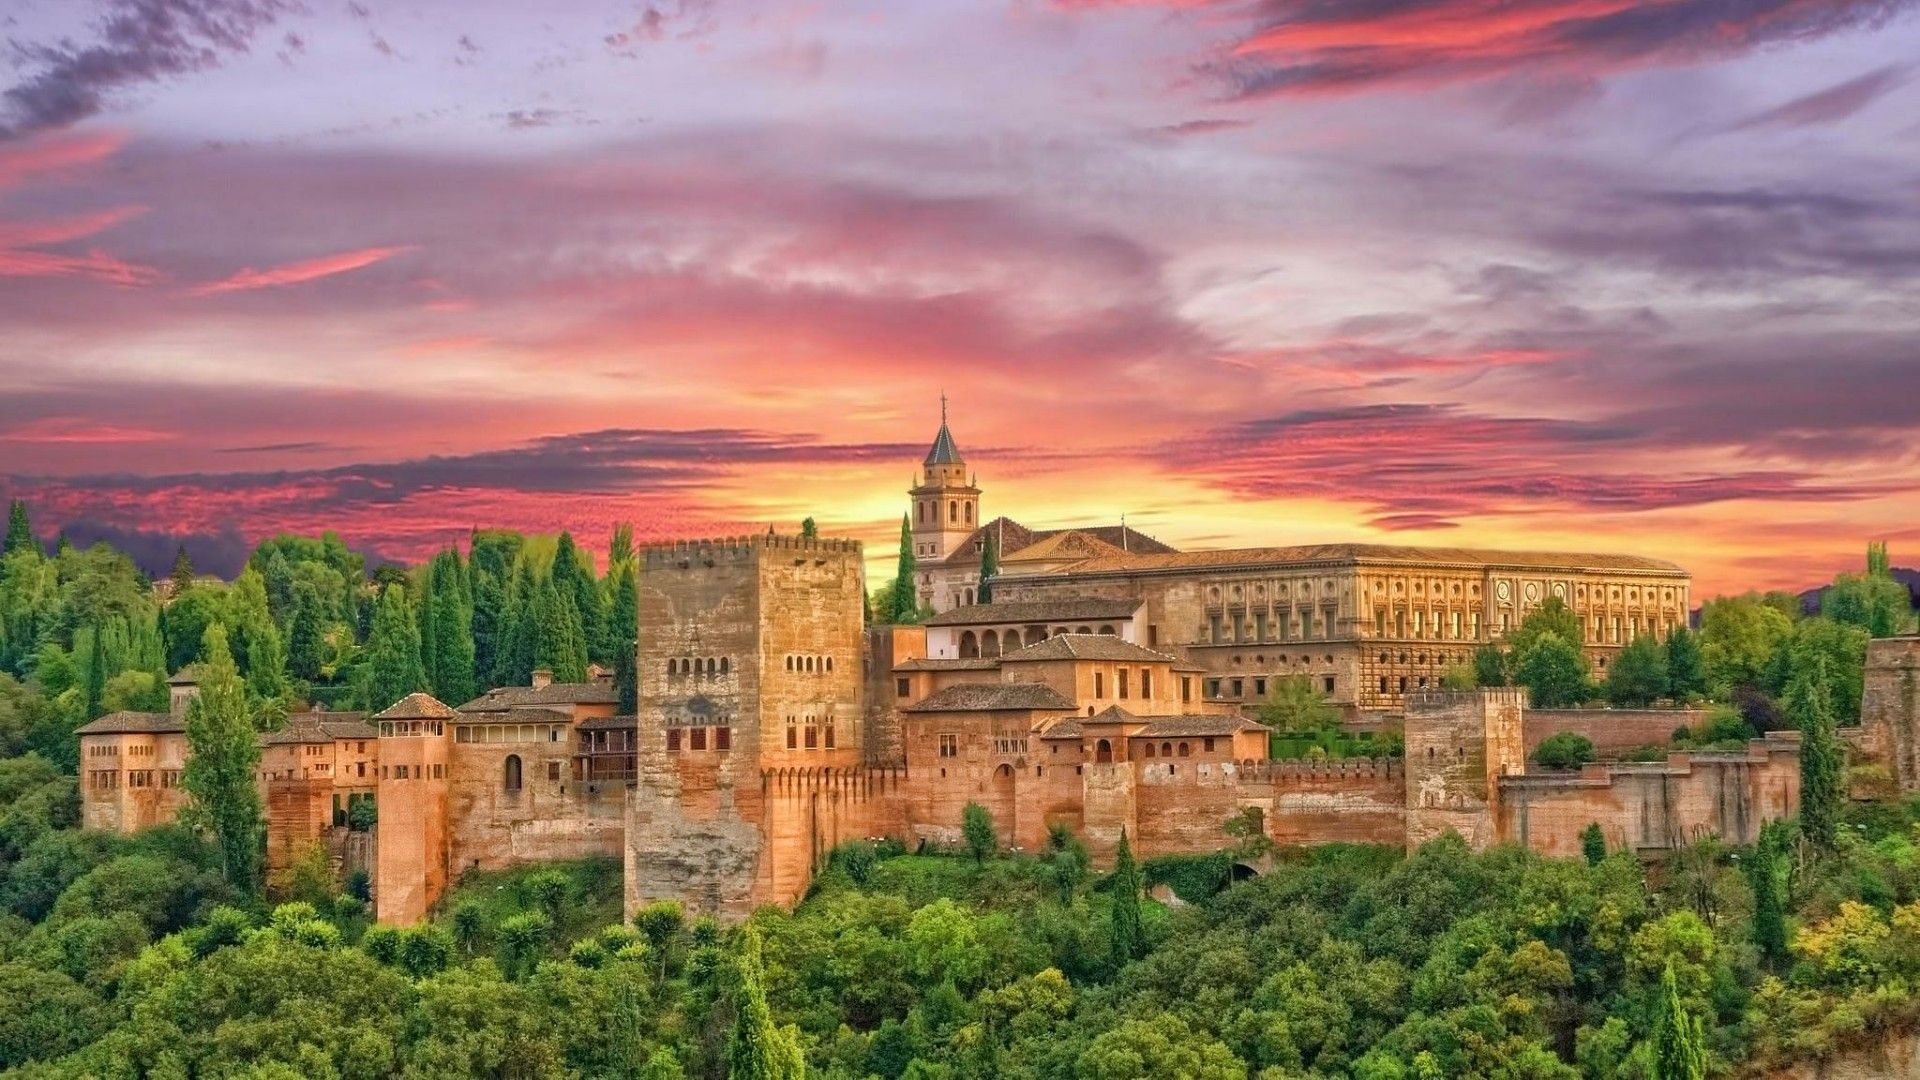
\includegraphics[width=\paperwidth,height=\paperheight,keepaspectratio]{images/granada.jpg}}
}

%comandos
\newcommand{\textorojo}[1]{\textbf{\textcolor{red}{#1}}}
\newcommand{\textoverde}[1]{\textbf{\textcolor{green}{#1}}}
\lstset{style=customcpp}

% Inicio del documento
% Inicio del documento
\begin{document}

% Portada
\maketitle
\thispagestyle{empty}

\begin{center}
    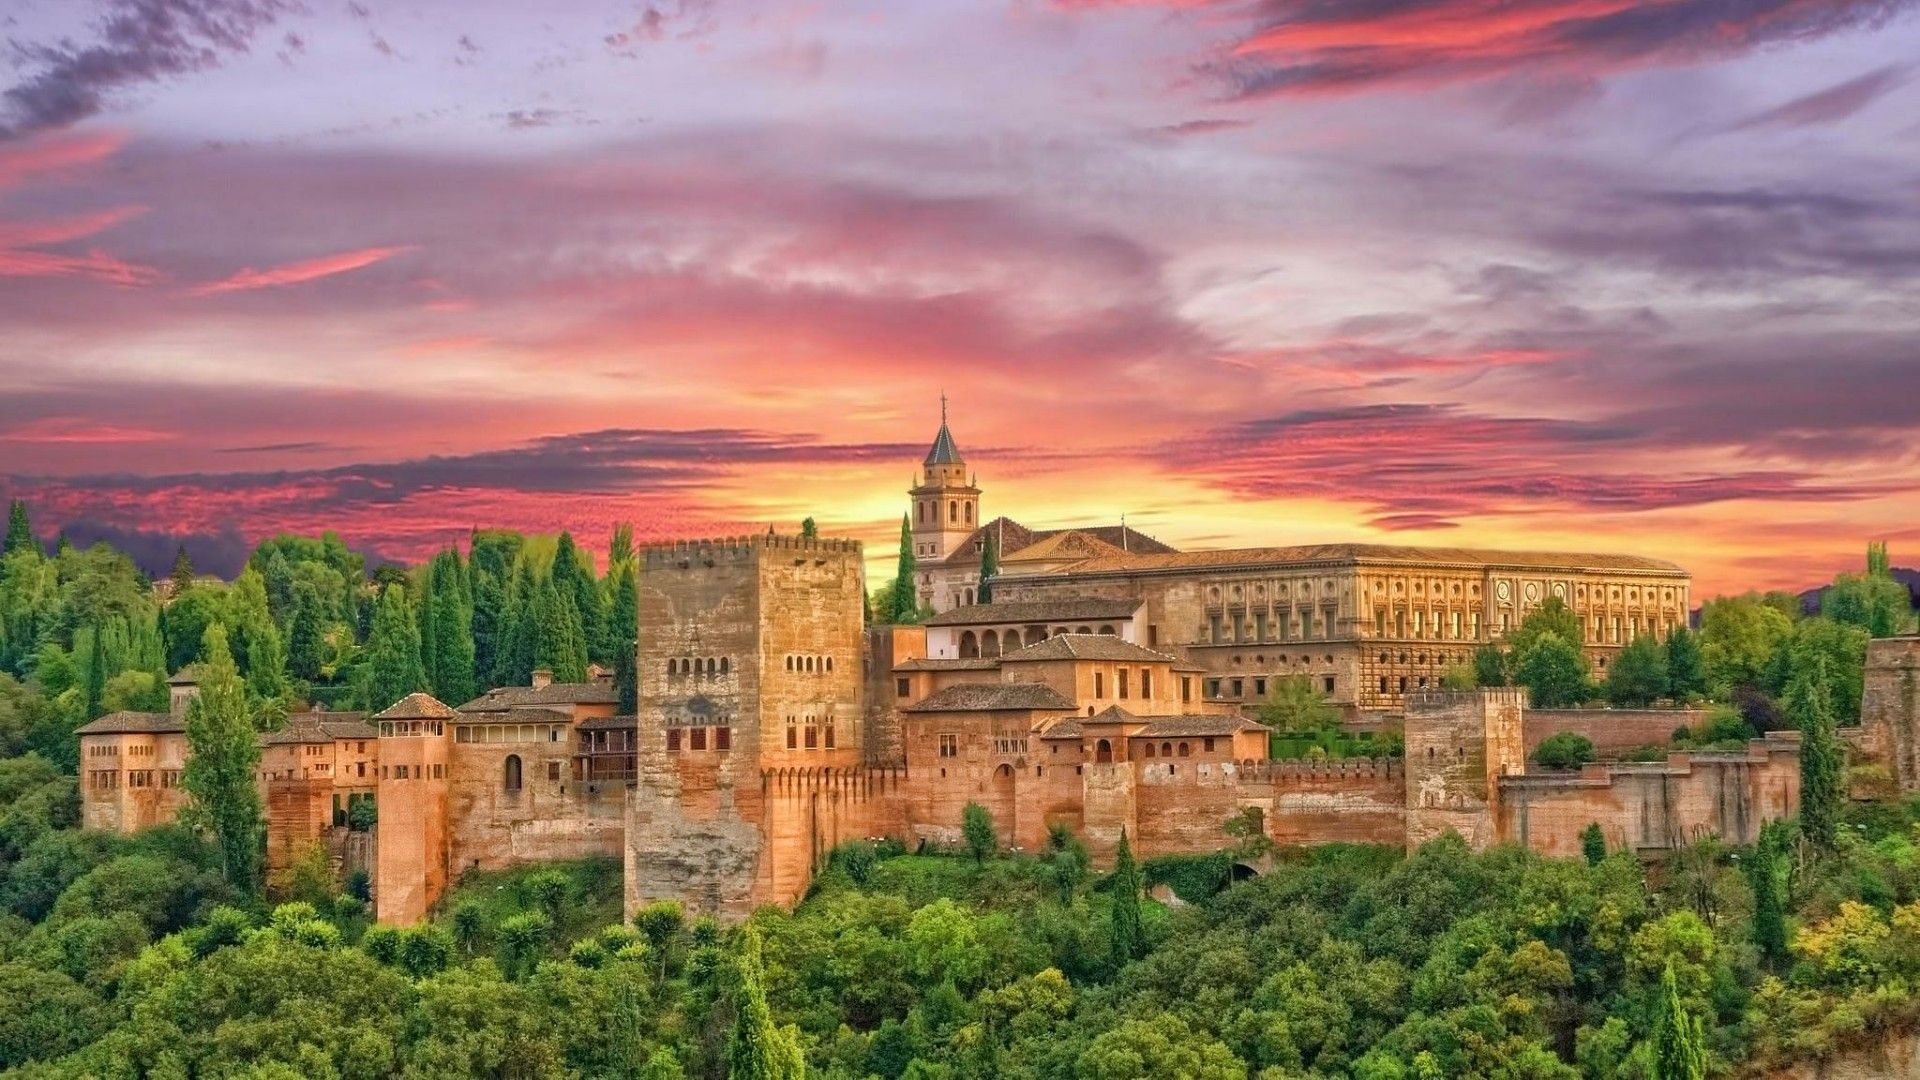
\includegraphics[width=\textwidth,height=0.4\textheight,keepaspectratio]{images/granada.jpg} \\ % Añade tu imagen de fondo
    \vfill
\end{center}

\newpage

% Índice
\tableofcontents
\newpage

\section{Ejemplo 1}

\begin{lstlisting}[style=customruby]
  # Definición de la clase Persona
  class Persona
    # Método initialize para inicializar la variable de instancia @nombre
    def initialize(n)
      @nombre = n # Se asigna el valor pasado al nombre de la persona
    end
  
    # Método andar que simula la acción de caminar
    def andar
      "Ando como una persona" # Devuelve una cadena describiendo la acción
    end
  
    # Método hablar que simula la acción de hablar
    def hablar
      "Hablo como una persona" # Devuelve una cadena describiendo cómo habla
    end
  end
  
  # Definición de la clase Profesor que hereda de Persona
  class Profesor < Persona
    # Sobrescribe el método hablar
    def hablar
      tmp = "Estimados alumnos:\n" # Cadena inicial específica para el profesor
      tmp += "Me llamo #{@nombre}\n" # Usa @nombre de la clase base Persona
      tmp += super # Llama al método hablar de la clase base
      tmp # Retorna la cadena completa
    end
  end
  
  # Crear una instancia de Profesor y llamar al método hablar
  puts Profesor.new("Jaime").hablar
  # Si Profesor no tiene un método initialize, usa el de Persona.
  # En este caso, @nombre es inicializado por el método initialize heredado.
  \end{lstlisting}
  
  \begin{itemize}
    \item \textbf{¿En qué momento ha tomado valor \texttt{@nombre}?}  
          La variable de instancia \texttt{@nombre} toma su valor al llamar al método \texttt{initialize} de la clase base \texttt{Persona} cuando se crea la instancia \texttt{Profesor.new("Jaime")}.
    \item \textbf{Si \texttt{Profesor} no tiene \texttt{initialize}, ¿qué va a ocurrir?}  
          Al no definir un método \texttt{initialize} propio, \texttt{Profesor} hereda el método \texttt{initialize} de \texttt{Persona}. Por lo tanto, \texttt{@nombre} será inicializado correctamente con el valor pasado al crear la instancia, en este caso, \texttt{"Jaime"}.
  \end{itemize}

\section{Ejemplo 2}

\begin{lstlisting}[style=customruby]
  # Definición de la clase A
  class A
    def initialize(a) # Método initialize con un argumento
      puts "Creando A" # Imprime un mensaje indicando que se crea A
      @a = a # Asigna el valor pasado a la variable de instancia @a
    end
  end
  
  # Definición de la clase B que hereda de A
  class B < A
  end
  
  # Crear una instancia de A con un argumento válido
  A.new(77) # Correcto: Se ejecuta initialize de A
  
  # Crear una instancia de B sin argumentos
  B.new # Incorrecto: No se pasa el argumento esperado por initialize de A
  
  # Crear una instancia de B con un argumento
  B.new(88) # Correcto: Se ejecuta initialize heredado de A con el argumento
  \end{lstlisting}
  
  \begin{itemize}
    \item Una de las 3 últimas líneas es errónea. ¿Cuál? ¿Por qué?  
          La línea \texttt{B.new} es errónea porque la clase \texttt{B} hereda el método \texttt{initialize} de \texttt{A}, que requiere un argumento. Sin ese argumento, se genera un error.
  \end{itemize}

\section{Ejemplo 3}
\begin{lstlisting}[style=customruby]
  # Definición de la clase C
  class C
    def initialize(c) # Método initialize con un argumento
      puts "Creando C" # Imprime un mensaje indicando que se crea C
      @c = c # Asigna el valor pasado a la variable de instancia @c
    end
  end
  
  # Definición de la clase D que hereda de C
  class D < C
    def initialize # Redefine el método initialize sin argumentos
      puts "Creando D" # Imprime un mensaje indicando que se crea D
      @d = 88 # Asigna 88 a la variable de instancia @d
    end
  end
  
  # Crear una instancia de C con un argumento válido
  C.new(99) # Correcto: Se ejecuta initialize de C con el argumento
  
  # Crear una instancia de D usando su initialize redefinido
  d = D.new # Correcto: Se ejecuta initialize de D
  
  # Mostrar el estado del objeto d
  puts d.inspect # Muestra las variables de instancia de d
  \end{lstlisting}
  
  \begin{itemize}
    \item ¿Qué ocurre en la línea 16?  
          Se crea una instancia de \texttt{D} y se ejecuta el método \texttt{initialize} redefinido en \texttt{D}. No se llama al método \texttt{initialize} de \texttt{C}.
    \item ¿Cuál es el resultado de la línea 17?  
          Muestra las variables de instancia del objeto \texttt{d}: \texttt{\("@d=>88\)}. La variable \texttt{@c} no existe porque no se llamó a \texttt{initialize} de \texttt{C}.
  \end{itemize}

\section{Ejemplo 4}
\begin{lstlisting}[style=customruby]
  # Definición de la clase E
  class E
    def initialize(e) # Método initialize con un argumento
      puts "Creando E" # Imprime un mensaje indicando que se crea E
      @e = e # Asigna el valor pasado a la variable de instancia @e
    end
  end
  
  # Definición de la clase F que hereda de E
  class F < E
    def initialize # Redefine initialize
      puts "Creando F" # Imprime un mensaje indicando que se crea F
      @f = 88 # Asigna 88 a la variable de instancia @f
      super(99) # Llama al initialize de E explícitamente con un argumento
    end
  end
  
  # Crear una instancia de E con un argumento válido
  E.new(99) # Correcto: Se ejecuta initialize de E
  
  # Crear una instancia de F usando su initialize redefinido
  f = F.new # Correcto: Se ejecuta initialize de F y también el de E
  
  # Mostrar el estado del objeto f
  puts f.inspect # Muestra las variables de instancia de f
  \end{lstlisting}
  
  \begin{itemize}
    \item ¿Qué ocurre en la línea 18?  
          Se crea una instancia de \texttt{F}, ejecutando primero el \texttt{initialize} de \texttt{F}, luego se llama explícitamente a \texttt{initialize} de \texttt{E} con \texttt{super(99)}.
    \item ¿Cuál es el resultado de la línea 19?  
          Muestra las variables de instancia del objeto \texttt{f}: \texttt{\("@f"=>88, "@e"=>99\)}. Ambas inicializaciones se completaron correctamente.
  \end{itemize}

  \begin{lstlisting}[style=customruby]
    # Definición de la clase G
    class G
      def initialize # Método initialize sin argumentos
        puts "Creando G" # Imprime un mensaje indicando que se crea G
        @g = 66 # Asigna 66 a la variable de instancia @g
      end
    end
    
    # Definición de la clase H que hereda de G
    class H < G
      def initialize # Redefine initialize sin llamar a super
        puts "Creando H" # Imprime un mensaje indicando que se crea H
        @h = 88 # Asigna 88 a la variable de instancia @h
      end
    end
    
    # Crear una instancia de G
    G.new # Correcto: Se ejecuta initialize de G
    
    # Crear una instancia de H usando su initialize redefinido
    h = H.new # Correcto: Se ejecuta initialize de H
    
    # Mostrar el estado del objeto h
    puts h.inspect # Muestra las variables de instancia de h
    \end{lstlisting}
    
    \begin{itemize}
      \item ¿Qué ocurre en la línea 16?  
            Se crea una instancia de \texttt{H}, ejecutando solo el método \texttt{initialize} redefinido en \texttt{H}. No se llama a \texttt{initialize} de \texttt{G}.
      \item ¿Cuál es el resultado de la línea 17?  
            Muestra las variables de instancia del objeto \texttt{h}: \texttt{\("@h"=>88\)}. La variable \texttt{@g} no existe porque no se llamó a \texttt{initialize} de \texttt{G}.
    \end{itemize}
    
  
  
  

\end{document}
